% pdflatex Dresden15
% $Author: predrag $ $Date: 2016-03-16 13:23:36 -0400 (Wed, 16 Mar 2016) $

%  talks/predrag/Dresden15/Dresden15.tex            2015-05-25
%  based on pipes/talks/Predrag/Marseille15/Marseille15.tex     2015-06-04

\input ../../inputs/layoutBeamer
\input ../../inputs/def % no edits, always from dasbuch/book/inputs
\input ../../inputs/defsBeamer

\title{\huge Turbulence, shmurbulence  \\ how fat is it?}
\author{P. Cvitanovi\'c}
\author[Cvitanovi\'c]
{
  \textcolor{green!50!black}{
  {Predrag~Cvitanovi\'c \\
  Xiong Ding, H. Chate, E. Siminos and K. A. Takeuchi
  }	%\inst{1}
  }
}
\institute
{
%  \inst{1}%
PDE Seminar, School of Mathematics \\
Georgia Institute of Technology
 }
\date{March 16, 2016}

\begin{document}

\begin{frame}
  \titlepage
\end{frame}


\section[what this talk is about]
 {what this talk is about}

\begin{frame}{part 1}
\begin{enumerate}
              \item {\Large
dynamical theory of turbulence
                  }\textcolor{gray}{\small
              \item
\statesp
              \item
symmetry reduction
              \item
dimension of the inertial manifold
                    }
            \end{enumerate}
\end{frame}


% \section[turbulence]
% {turbulence}

\begin{frame}{a life in extreme dimensions}
\begin{block}{since 1822 have Navier-Stokes equations}
\[
\dfrac{\partial \bv}{\partial t} + (\bv \cdot \nabla) \bv
	\,=\,
\frac{1}{R} \nabla ^2 \bv
-\nabla p
+ \mathbf{f}
    \,,\qquad
\nabla \cdot \bv = 0,
\]
\end{block}

\hfill{\small
velocity field  $\bv \in \mathbb{R}^3$
;
pressure field $p$
;
driving force $\mathbf{f}$
        }

\medskip

\begin{block}{since  1883 Osborne Reynolds experiments}
an outstanding problem of classical physics :
\end{block}

\bigskip

% large Reynolds number $R$:
\hfill {\Large\textcolor{red}{describe turbulence}}

\end{frame}

\begin{frame}{plane Couette experiment}
\begin{center}
\includegraphics[width=1.0\textwidth]{planeCouette}
\end{center}
B. Hof lab
\end{frame}

\begin{frame}{pipe experiment}
\begin{center}
\includegraphics[width=0.28\textwidth]{pipe}
\end{center}
B. Hof lab
\end{frame}

\begin{frame}{pipe experiment data point}
\begin{block}{a state of turbulent pipe flow at instant in time}
\end{block}

\bigskip

%%%%%%%%%%%%%%%%%%%%%%%%%%%%%%%%%%%%%%%%%%%%%%%%%%%%%%%%%%%%%%%%%%
%\hfill
%\begin{minipage}[c]{0.35\textwidth}
Stereoscopic Particle Image Velocimetry $\to$
3-$d$ velocity field over the entire pipe%
\footnote{
%"Stereoscopic PIV on transition in pipe flow",
Casimir W.H. van Doorne
(PhD thesis, Delft  2004)
%; 	{\tt www.ahd.tudelft.nl}
}

\bigskip

\begin{center}
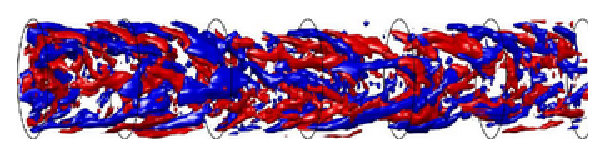
\includegraphics[width=0.90\textwidth]{vDoorne4}
\end{center}
\end{frame}


\begin{frame}{numerical challenges}
		\only<1-2>{
            \begin{block}{computation of turbulent solutions}
requires 3-dimensional volume discretization
\\
$\to$ integration of  $10^4$-$10^6$ coupled ordinary differential equations

\bigskip

challenging, but today possible


\bigskip
        }
		\only<1-2>{
J.F. Gibson
\HREF{http://channelflow.org/}{ChannelFlow.org}
\\
A. P. Willis
\HREF{http://www.openpipeflow.org/}{OpenPipeFlow.org}
            \end{block}
        }
		\only<2>{
            \begin{block}{typical simulation}
each instant of the flow $ > $ Megabytes
\\
a video of the flow $> $ Gigabytes
            \end{block}
                }
\end{frame}

\begin{frame}{example : pipe flow}
amazing data! amazing numerics!
\begin{center}
  \includegraphics[width=1.0\textwidth,clip=true]
                    {pipeSects}
\end{center}

\begin{itemize}
 \item here each instant of the flow $\approx$ 2.5\,MB
 \item videos of the flow $\approx$ GBs
\end{itemize}
\end{frame}

\begin{frame}{plane Couette velocity visualization}
\begin{center}
\includegraphics[width=1.0\textwidth]{bigbox}
\end{center}
\end{frame}

\begin{frame}{computational cell, velocity visualization}
\begin{center}
\includegraphics[width=0.5\textwidth]{statseSpProj3center}
\end{center}
next - the same solution, different visualization
\end{frame}

\begin{frame}{plane Couette isovorticity visualization}
\begin{center}
\includegraphics[width=1.0\textwidth]{ItGe09}
\end{center}
\end{frame}


\begin{frame}{part 2}
\begin{enumerate}
              \item
    \textcolor{gray}{\small
dynamical theory of turbulence
        }
              \item
    {\Large
\statesp
    }\textcolor{gray}{\small
              \item
symmetry reduction
              \item
dimension of the inertial manifold
                    }
            \end{enumerate}
\end{frame}


\section[dynamics in $\infty$ dimensions]
{dynamics in $\infty$ dimensions}

\begin{frame}{new : look at it in}
\bigskip
\hfill
{\Huge \statesp!}
\vfill
E. Hopf 1948
\end{frame}

\begin{frame}{dynamical description of turbulence}
%	from {../chapter/dynsysII}

\begin{block}{\statesp}
a manifold $\pS \in \reals^{d}$ :
$d$ numbers determine the state of the system
\end{block}

\bigskip

\begin{block}{representative point }
$\ssp(t) \in \pS$
\\
a state of physical system at instant in time
\end{block}

\bigskip

\begin{block}{deterministic dynamics}
trajectory $\ssp(\zeit) = \flow{\zeit}{\xInit}$ =
representative point time $\zeit$ later
\end{block}
\end{frame}

\begin{frame}{today's experiments}
\begin{block}{example of a representative point }
$\ssp(t) \in \pS$, $d= \infty$ \\
a state of turbulent pipe flow at instant in time
\end{block}

\bigskip

%%%%%%%%%%%%%%%%%%%%%%%%%%%%%%%%%%%%%%%%%%%%%%%%%%%%%%%%%%%%%%%%%%
%\hfill
%\begin{minipage}[c]{0.35\textwidth}
Stereoscopic Particle Image Velocimetry $\to$
3-$d$ velocity field over the entire pipe%
\footnote{
%"Stereoscopic PIV on transition in pipe flow",
Casimir W.H. van Doorne
(PhD thesis, Delft  2004)
%; 	{\tt www.ahd.tudelft.nl}
}

\bigskip

\begin{center}
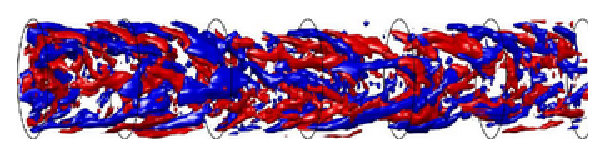
\includegraphics[width=0.90\textwidth]{vDoorne4}
\end{center}
\end{frame}

\begin{frame}{charting the state space of a turbulent flow}
John F Gibson (U New Hampshire)
\\
Jonathan Halcrow (Google)
\end{frame}

\begin{frame}{can visualize 61,506 dimensional \statesp\ of turbulent flow}
\begin{center}
\includegraphics[width=0.80\textwidth]{NCC1701b}
\end{center}
\eqva\ of turbulent plane Couette flow,
\\
their unstable manifolds, and
\\
myriad of turbulent videos mapped out as one happy family

\bigskip

\hfill   {\small
          for movies, please click through
            \textcolor{blue}{\href{http://ChaosBook.org/tutorials}
             {ChaosBook.org/tutorials}}
          }
\end{frame}

\begin{frame}{plane Couette state space, an \eqv\ unstable manifold}
\begin{center}
\includegraphics[width=0.6\textwidth]{ubfp_unstab_trajs}
\end{center}
\end{frame}

\begin{frame}{plane Couette state space $10^5 \to 3D$}
\begin{center}
\includegraphics[width=0.8\textwidth]{a1_14_g2}
\end{center}
\end{frame}


%%%%%%%%%%%%%%%%%%%%%%%%%%%%%%%%%%%%%%%%%%%%%%%%%%%%%%%%%%%%%%%%%%%%%%%%%%%%
\section[who's afraid of symmetry]{who's afraid of symmetry}

\begin{frame}{part 3}
\begin{enumerate}
              \item
    \textcolor{gray}{\small
dynamical theory of turbulence
              \item
\statesp
        }
              \item
    {\Large
symmetry reduction
    }\textcolor{gray}{\small
              \item
dimension of the inertial manifold
                    }
            \end{enumerate}
\end{frame}


\begin{frame}{}
\begin{block}{}
{\Huge
nature loves symmetry
}
\end{block}
or does she?

\bigskip\bigskip\bigskip

\begin{block}{\Large problem}
    {\large
physicists like symmetry more than Nature
    }

\bigskip

\hfill
Rich Kerswell
\end{block}
\end{frame}

\begin{frame}{nature : turbulence in pipe flows}
\begin{tabbing}
bottom \= : \= experimental / numerical data \kill
  % \> for next tab, \\ for new line...
~~top~ \> : \> experimental / numerical data \\
bottom \> : \> theorist's solutions
\end{tabbing}
\begin{center}
  \includegraphics[width=1.0\textwidth,clip=true]
                    {pipeSects}
\end{center}

\bigskip
Nature, \textcolor{red}{she don't care} :
turbulence breaks all symmetries
\end{frame}

\begin{frame}{in turbulence, }
use of {\Large symmetries is subtle}

\vfill
Elie Cartan 1926 :
\hfill
{\Large slice it!}
\end{frame}

\begin{frame}{example : $\SOn{2}_z\times \On{2}_\theta$ symmetry of pipe flow}
            \begin{block}{}
 %% A27*-pipeSymms.* - read dasbuch/book/FigSrc/inkscape/00ReadMe.txt
 \begin{center}
  \setlength{\unitlength}{0.35\textwidth}
  %% \unitlength = units used in the Picture Environment
(a)
  \begin{picture}(1,0.52454249)%
    \put(0,0){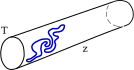
\includegraphics[width=\unitlength]{A27a-pipeSymms}}%
    \put(0.61583231,0.13683004){\color[rgb]{0,0,0}\makebox(0,0)[lb]{\smash{$z$}}}%
    \put(0.00611823,0.27217453){\color[rgb]{0,0,0}\makebox(0,0)[lb]{\smash{$\theta$}}}%
  \end{picture}%
(b)
  \begin{picture}(1,0.52454249)%
    \put(0,0){\includegraphics[width=\unitlength]{A27b-pipeSymms}}%
    \put(0.61583231,0.13683004){\color[rgb]{0,0,0}\makebox(0,0)[lb]{\smash{$z$}}}%
    \put(0.00611823,0.27217453){\color[rgb]{0,0,0}\makebox(0,0)[lb]{\smash{$\theta$}}}%
  \end{picture}%
\\
(c)
  \begin{picture}(1,0.52454249)%
    \put(0,0){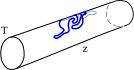
\includegraphics[width=\unitlength]{A27c-pipeSymms}}%
    \put(0.61583231,0.13683004){\color[rgb]{0,0,0}\makebox(0,0)[lb]{\smash{$z$}}}%
    \put(0.00611823,0.27217453){\color[rgb]{0,0,0}\makebox(0,0)[lb]{\smash{$\theta$}}}%
  \end{picture}%
(d)
  \begin{picture}(1,0.52454249)%
    \put(0,0){\includegraphics[width=\unitlength]{A27d-pipeSymms}}%
    \put(0.61583231,0.13683004){\color[rgb]{0,0,0}\makebox(0,0)[lb]{\smash{$z$}}}%
    \put(0.00611823,0.27217453){\color[rgb]{0,0,0}\makebox(0,0)[lb]{\smash{$\theta$}}}%
  \end{picture}%
 \end{center}
a fluid state, shifted by a stream-wise translation, azimuthal rotation
$g_p$ is a physically equivalent state
			\end{block}
%	\end{columns}
% \caption{\label{fig:A27-pipeSymms}
			\begin{exampleblock}{}
\begin{itemize}
  \item[b)]  stream-wise
  \item[c)]  stream-wise, azimuthal
  \item[d)]  azimuthal flip
\end{itemize}
			\end{exampleblock}
\end{frame}

\begin{frame}{\statesp\ trajectories, group orbits}
%  \caption{\label{fig:A27wurst} from atlas12
  \setlength{\unitlength}{0.28\textwidth}
\begin{center}
{\scriptsize %small
(a)
  \begin{picture}(1,0.98239821)%
    \put(0,0){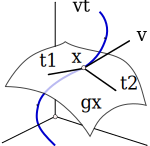
\includegraphics[width=\unitlength]{A28tangent3}}%
    \put(0.91612064,0.70682767){\color[rgb]{0,0,0}\makebox(0,0)[lb]{\smash{$\vel$}}}%
    \put(0.48698745,0.90266503){\color[rgb]{0,0,0}\makebox(0,0)[lb]{\smash{$\ssp(\zeit)$}}}%
    \put(0.2624318,0.5347756){\color[rgb]{0,0,0}\makebox(0,0)[lb]{\smash{$\groupTan_1$}}}%
    \put(0.80471037,0.38188675){\color[rgb]{0,0,0}\makebox(0,0)[lb]{\smash{$\groupTan_2$}}}%
    \put(0.538343,0.25344355){\color[rgb]{0,0,0}\makebox(0,0)[lb]{\smash{$\pS_\ssp$}}}%
    \put(0.47864531,0.56060893){\color[rgb]{0,0,0}\makebox(0,0)[lb]{\smash{$\ssp$}}}%
  \end{picture}%
~~~~~~~(b)
  \begin{picture}(1,0.9071451)%
    \put(0,0){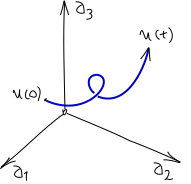
\includegraphics[width=\unitlength]{A27traj}}%
    \put(0.81413243,0.74633551){\color[rgb]{0,0,0}\makebox(0,0)[lb]{\smash{$\ssp(\zeit)$}}}%
    \put(0.14085867,0.30233715){\color[rgb]{0,0,0}\makebox(0,0)[lb]{\smash{$\ssp(0)$}}}%
  \end{picture}%
\\
(c)
	\begin{picture}(1,0.88265338)%
    \put(0,0){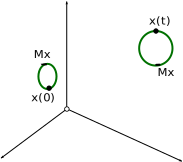
\includegraphics[width=\unitlength]{A27gOrbit}}%
    \put(0.17017404,0.30123416){\color[rgb]{0,0,0}\makebox(0,0)[lb]{\smash{$\ssp(0)$}}}%
    \put(0.10473094,0.59736144){\color[rgb]{0,0,0}\makebox(0,0)[lb]{\smash{$\pS_{\ssp(0)}$}}}%
    \put(0.80073137,0.42842331){\color[rgb]{0,0,0}\makebox(0,0)[lb]{\smash{$\pS_{\ssp(\zeit)}$}}}%
    \put(0.81421682,0.75061198){\color[rgb]{0,0,0}\makebox(0,0)[lb]{\smash{$\ssp(\zeit)$}}}%
	\end{picture}%
~~~~~~~(d)
	\begin{picture}(1,0.90708568)%
    \put(0,0){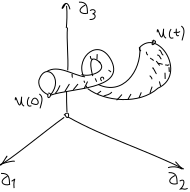
\includegraphics[width=\unitlength]{A27wurst}}%
    \put(0.81871555,0.75240026){\color[rgb]{0,0,0}\makebox(0,0)[lb]{\smash{$\ssp(\zeit)$}}}%
    \put(0.12337724,0.29209515){\color[rgb]{0,0,0}\makebox(0,0)[lb]{\smash{$\ssp(0)$}}}%
	\end{picture}%
} %end {\small
\end{center}

	\begin{columns}[t]
	\column{.65\textwidth}
(a) $\ssp$ tangent vectors:

\medskip

$\vel(\ssp)$ along time flow $\ssp(\zeit)$
\\
$\groupTan_1(\ssp),\, \cdots, \groupTan_N(\ssp)$
group tangents
	\column{.35\textwidth}
%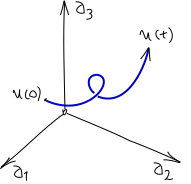
\includegraphics[width=0.95\textwidth]{A27traj}
(b) trajectory $\ssp(\zeit)$
%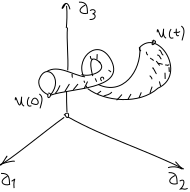
\includegraphics[width=0.95\textwidth]{A27wurst}

\medskip

%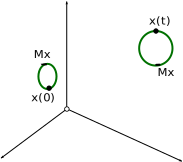
\includegraphics[width=0.95\textwidth]{A27gOrbit}
(c) group orbits $\LieEl\,\ssp(\zeit)$

\medskip

(d) wurst $\LieEl\,\ssp(\zeit)$
	\end{columns}
\end{frame}

\begin{frame}{\rpo, in full \statesp\ and in \slice}
\begin{center}
\includegraphics[width=0.45\textwidth]{BBO2a1045rpossp}
\includegraphics[width=0.45\textwidth]{BBO2a1045rposlice}
\end{center}
\end{frame}


\section[relativity for cyclists]{relativity for cyclists}

\subsection[in/equivariance]{}

\begin{frame}{foliation by group orbits}
  \begin{columns}
  \column{0.5\textwidth}
\begin{block}{}
% 2011-08-23 Predrag: previously BeThTraj.pdf from
% dasbuch/book/FigSrc/inkscape/BeThTraj.svg
%  2011-09-09 Predrag: updated continuous.tex overheads
%  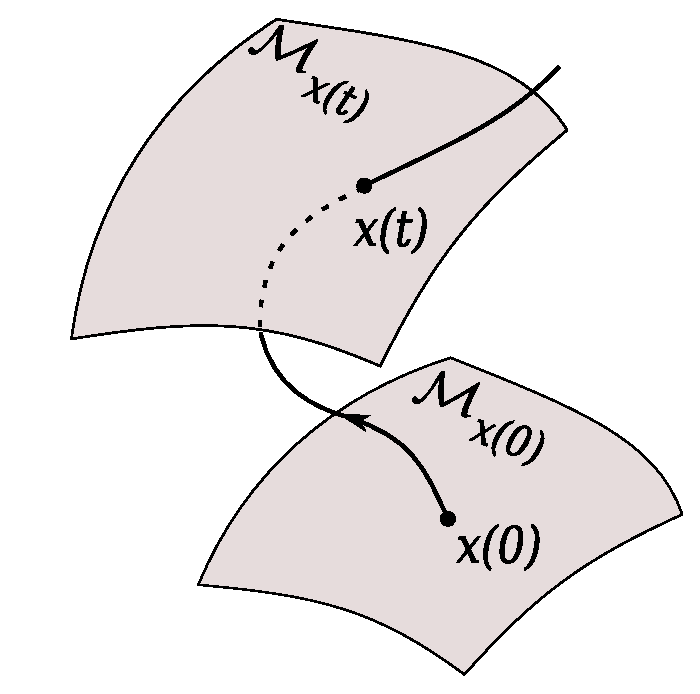
\includegraphics[width=1.00\textwidth,clip=true]{BeThTraj}
 \begin{center}
  \setlength{\unitlength}{1.00\textwidth}
  %% \unitlength = units used in the Picture Environment
  {\scriptsize
\only<1-2>{
  \begin{picture}(1,0.98655417)%
    \put(0,0){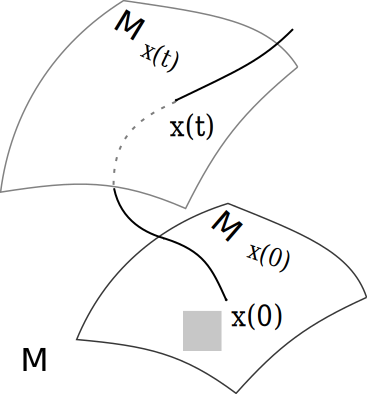
\includegraphics[width=\unitlength]{BeThTrajTeX}}%
    \put(0.35976094,0.91875614){\color[rgb]{0,0,0}\rotatebox{-16.32889204}{\makebox(0,0)[lb]{\smash{$\pS_{\ssp(\zeit)}$}}}}%
        \put(0.60333631,0.42274457){\color[rgb]{0,0,0}\rotatebox{-30.8073288}{\makebox(0,0)[lb]{\smash{$\pS_{\ssp(0)}$}}}}%
    \put(0.63001383,0.14959019){\color[rgb]{0,0,0}\rotatebox{0.0313674}{\makebox(0,0)[lb]{\smash{$\ssp(0)$}}}}%
    \put(0.4558276,0.64524238){\color[rgb]{0,0,0}\rotatebox{0.0313674}{\makebox(0,0)[lb]{\smash{$\ssp(\zeit)$}}}}%
    \put(0.13110825,0.05766516){\color[rgb]{0,0,0}\rotatebox{0.11031334}{\makebox(0,0)[lb]{\smash{$\pS$}}}}%
  \end{picture}%
  }
\only<3>{
  \begin{picture}(1,0.97809647)%
    \put(0,0){\includegraphics[width=\unitlength]{BeThFoliTeX}}%
    \put(0.35673326,0.91086901){\color[rgb]{0,0,0}\rotatebox{-31.32889204}{\makebox(0,0)[lb]{\smash{$\pS_{\ssp(\zeit)}$}}}}%
    \put(0.8041738,0.27513933){\color[rgb]{0,0,0}\rotatebox{-40.8073288}{\makebox(0,0)[lb]{\smash{$\pS_{\ssp(0)}$}}}}%
    \put(0.64701656,0.09606165){\color[rgb]{0,0,0}\rotatebox{0.0313674}{\makebox(0,0)[lb]{\smash{$\ssp(0)$}}}}%
    \put(0.50157066,0.63965709){\color[rgb]{0,0,0}\rotatebox{0.0313674}{\makebox(0,0)[lb]{\smash{$\ssp(\zeit)$}}}}%
    \put(0.13000487,0.05702481){\color[rgb]{0,0,0}\rotatebox{0.11031334}{\makebox(0,0)[lb]{\smash{$\pS$}}}}%
  \end{picture}%
  }
  } % end {\scriptsize
 \end{center}
\end{block}
  \column{0.5\textwidth}
		\only<1>{
\noindent
\emph{group orbit} $\pS_\ssp $ of $\ssp$ is the set of all group
actions
\[
\pS_\ssp = \{\LieEl\,\ssp \mid \LieEl \in {\Group}\}
\]
        }
		\only<2>{
%\noindent
%group orbit $\pS_{\ssp(0)}$ of \statesp\ point
% $\ssp(0)$, and the group orbit $\pS_{\ssp(\zeit)}$
%reached by the trajectory $\ssp(\zeit)$ time $t$ later.
%        }
%		\only<3>{
\noindent
any point on the manifold $\pS_{\ssp(\zeit)}$ is
equivalent to any other
        }
		\only<3>{
\noindent
actions of a symmetry group
foliates the \statesp\ $\pS$ into a union of group
orbits $\pS_{\ssp}$

\medskip

each group orbit $\pS_{\ssp}$ is an equivalence class
        }
\end{columns}
\end{frame}

\section{symmetry reduction}

\begin{frame}{}
\begin{block}{the goal}
replace each group orbit by a unique
point in a lower-dimensional

\bigskip

\hfill
\textcolor{red}{\Large symmetry \reducedsp\ $\pS/\Group$}
\end{block}
\end{frame}


\begin{frame}{} %symmetry reduction}
  \begin{columns}
  \column{0.48\textwidth}
\begin{block}{full \statesp}
\bigskip
 \begin{center}
  \setlength{\unitlength}{1.00\textwidth}
  %% \unitlength = units used in the Picture Environment
  \begin{picture}(1,0.98655417)%
    \put(0,0){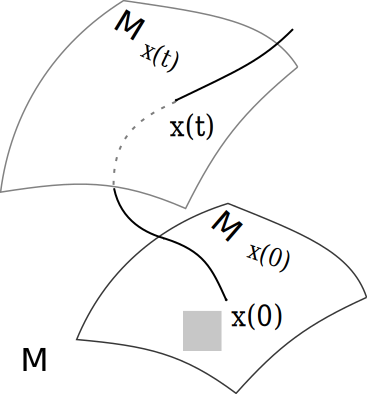
\includegraphics[width=\unitlength]{BeThTrajTeX}}%
    \put(0.35976094,0.91875614){\color[rgb]{0,0,0}\rotatebox{-16.32889204}{\makebox(0,0)[lb]{\smash{$\pS_{\ssp(\zeit)}$}}}}%
        \put(0.60333631,0.42274457){\color[rgb]{0,0,0}\rotatebox{-30.8073288}{\makebox(0,0)[lb]{\smash{$\pS_{\ssp(0)}$}}}}%
    \put(0.63001383,0.14959019){\color[rgb]{0,0,0}\rotatebox{0.0313674}{\makebox(0,0)[lb]{\smash{$\ssp(0)$}}}}%
    \put(0.4558276,0.64524238){\color[rgb]{0,0,0}\rotatebox{0.0313674}{\makebox(0,0)[lb]{\smash{$\ssp(\zeit)$}}}}%
    \put(0.13110825,0.05766516){\color[rgb]{0,0,0}\rotatebox{0.11031334}{\makebox(0,0)[lb]{\smash{$\pS$}}}}%
  \end{picture}%
 \end{center}
\end{block}
  \column{0.45\textwidth}
\begin{block}{\reducedsp}
\bigskip
 \begin{center}
  \setlength{\unitlength}{1.00\textwidth}
  %% \unitlength = units used in the Picture Environment
  \begin{picture}(1,1.07315413)%
    \put(0,0){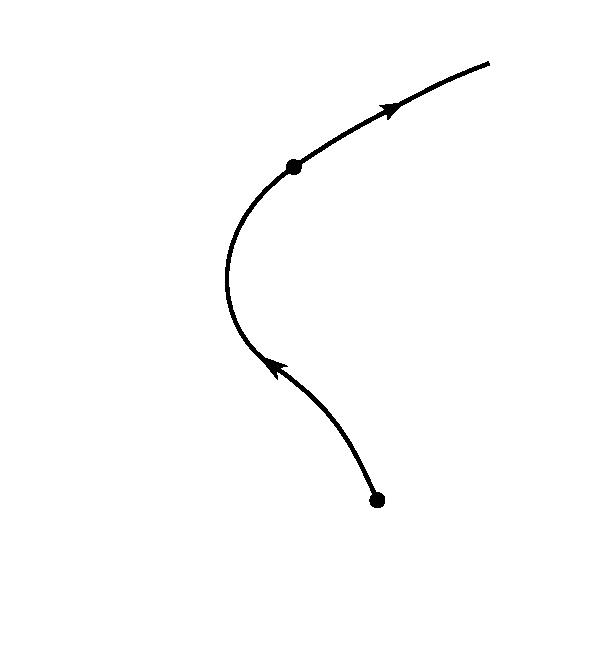
\includegraphics[width=\unitlength]{BeThRedTeX}}%
    \put(0.19912369,0.17144733){\color[rgb]{0,0,0}\rotatebox{0.11031334}{\makebox(0,0)[lb]{\smash{$\pSRed$}}}}%
    \put(0.63028127,0.18433598){\color[rgb]{0,0,0}\rotatebox{0.03136739}{\makebox(0,0)[lb]{\smash{$\sspRed(0)$}}}}%
    \put(0.46253394,0.70182305){\color[rgb]{0,0,0}\rotatebox{0.03136739}{\makebox(0,0)[lb]{\smash{$\sspRed(\tau)$}}}}%
  \end{picture}%
 \end{center}
\end{block}
\end{columns}
\begin{block}{}
replace each group orbit by a unique
point in a lower-dimensional

\bigskip

\hfill
\textcolor{red}{\Large symmetry \reducedsp\ $\pS/\Group$}
\end{block}
\end{frame}

\begin{frame}{symmetry reduction : how?}

\begin{block}{continuous symmetry reduction in high-dimensional flows}
{with }
\bigskip

%\label{fig:A27movFrame}
\hfill {\Huge  the method of slices}
\end{block}
\end{frame}



% \subsection[slice n' dice]{slice n' dice}

\begin{frame}{Cartan's idea : moving frame}
  \begin{columns}
  \column{0.50\textwidth}
\begin{block}{}
%\label{fig:A27movFrame}
 \begin{center}
  \setlength{\unitlength}{0.80\textwidth}
  %% \unitlength = units used in the Picture Environment
{\scriptsize %small
%(a)~~
  \begin{picture}(1,0.98655417)%
    \put(0,0){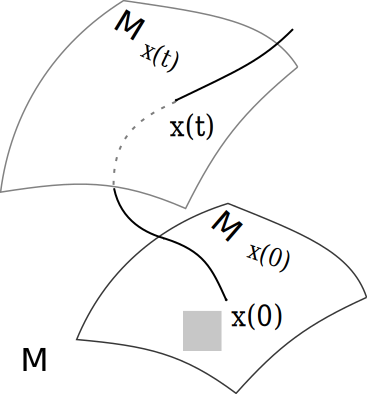
\includegraphics[width=\unitlength]{BeThTrajTeX}}%
    \put(0.35976094,0.91875614){\color[rgb]{0,0,0}\rotatebox{-16.32889204}{\makebox(0,0)[lb]{\smash{$\pS_{\ssp(\zeit)}$}}}}%
        \put(0.60333631,0.42274457){\color[rgb]{0,0,0}\rotatebox{-30.8073288}{\makebox(0,0)[lb]{\smash{$\pS_{\ssp(0)}$}}}}%
    \put(0.63001383,0.14959019){\color[rgb]{0,0,0}\rotatebox{0.0313674}{\makebox(0,0)[lb]{\smash{$\ssp(0)$}}}}%
    \put(0.4558276,0.64524238){\color[rgb]{0,0,0}\rotatebox{0.0313674}{\makebox(0,0)[lb]{\smash{$\ssp(\zeit)$}}}}%
    \put(0.13110825,0.05766516){\color[rgb]{0,0,0}\rotatebox{0.11031334}{\makebox(0,0)[lb]{\smash{$\pS$}}}}%
  \end{picture}%
}% end {\scriptsize %small
 \end{center}
\end{block}
  \column{0.50\textwidth}
\begin{block}{}
%\label{fig:A27movFrame}
 \begin{center}
  \setlength{\unitlength}{0.80\textwidth}
  %% \unitlength = units used in the Picture Environment
{\scriptsize %small
%(b)
  \begin{picture}(1,0.98742208)%
    \put(0,0){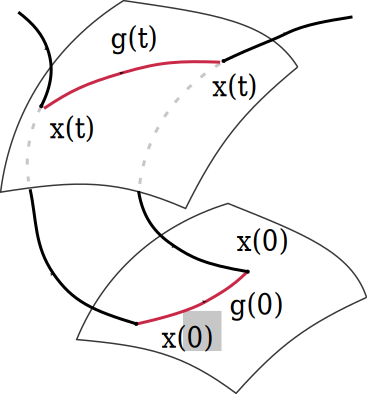
\includegraphics[width=\unitlength]{BeThMovFr}}%
    \put(0.20546387,0.64069775){\color[rgb]{0,0,0}\rotatebox{0.0313674}{\makebox(0,0)[lb]{\smash{$\ssp(\zeit)$}}}}%
    \put(0.7334028,0.27844745){\color[rgb]{0,0,0}\rotatebox{0.0313674}{\makebox(0,0)[lb]{\smash{$\sspRed(0)$}}}}%
    \put(0.52082757,0.7302884){\color[rgb]{0,0,0}\rotatebox{0.0313674}{\makebox(0,0)[lb]{\smash{$\sspRed(\zeit)$}}}}%
    \put(0.35738205,0.88152375){\color[rgb]{0,0,0}\rotatebox{0.0313674}{\makebox(0,0)[lb]{\smash{$\LieEl(\zeit)$}}}}%
    \put(0.48490227,0.11640486){\color[rgb]{0,0,0}\rotatebox{0.0313674}{\makebox(0,0)[lb]{\smash{$\ssp(0)$}}}}%
    \put(0.3947908,0.25892637){\color[rgb]{0,0,0}\rotatebox{0.0313674}{\makebox(0,0)[lb]{\smash{$\LieEl(0)$}}}}%
    \put(0.1047908,0.0792637){\color[rgb]{0,0,0}\rotatebox{0.0313674}{\makebox(0,0)[lb]{\smash{$\pS$}}}}%
  \end{picture}%
}% end {\scriptsize %small
 \end{center}
\end{block}
	\end{columns}

\bigskip

free to redefine the flow any time instant \\ by transformation to \\
a frame moving
along symmetry directions
\end{frame}



\section[slice n' dice]{slice n' dice}

\begin{frame}{relativity for cyclists}
\begin{block}{\mslices}

\bigskip
cut group orbits by a hypersurface
\textcolor{red}{(not a Poincar\'e section)}, each group orbit of
symmetry-equivalent points represented by the single point
\end{block}
\bigskip
\textcolor{blue}{\Large cut how?}
\bigskip\bigskip
\begin{block}{geometers'choice}
chose the frames so that distances are minimized
\end{block}
\end{frame}

\section{slice \& dice}

\begin{frame}{\rpo, in full \statesp\ and in \slice}
\begin{center}
\includegraphics[width=0.45\textwidth]{BBO2a1045rpossp}
\includegraphics[width=0.45\textwidth]{BBO2a1045rposlice}
\end{center}
\end{frame}

\begin{frame}{group orbits are NOT circles}
\begin{block}{nonlinearities couple many Fourier modes}
group orbit manifolds of highly nonlinear states are smooth, but not nice
\end{block}
\end{frame}


\begin{frame}{example : group orbit of a pipe flow turbulent state}
%\slicep\ is Kerswell \emph{et al} $N2\_M1$  \reqv
%\\
%( $\Reynolds =2400$,
%stubby $L=2.5D$ pipe)
	\begin{columns}[t]
	\column{.45\textwidth}
			\begin{exampleblock}
{$\SOn{2}\times\SOn{2}$ symmetry
\\
$\Rightarrow$
group orbit is
\\
topologically 2-torus,
\\ but
\\
a mess in any projection}
			\end{exampleblock}
	\column{0.55\textwidth}
\begin{block}
  \centering
\includegraphics[width=1.00\textwidth]{2840GOt135M1} %{2830GO7}
%  \caption{\label{fig:2830GO6}
    %\label{fig:M1groupOrb}
\end{block}
	\end{columns}

\bigskip
group orbits of highly nonlinear states are topologically tori,
but highly contorted tori

\vfill
\hfill
Ashley Willis
\end{frame}

\begin{frame}{example : pipe flow \rpo}
  \begin{columns}
  \column{0.48\textwidth}
\begin{block}{3 repeats, full space}
\includegraphics[width=1.00\textwidth,clip=true]{2841GO3a}%
\end{block}
  \column{0.48\textwidth}
\begin{block}{reduced space}
\includegraphics[width=1.00\textwidth,clip=true]{2841GO3b}%
\end{block}
  \end{columns}
\vfill
%\hfill
Ashley Willis
\end{frame}

\section[Das Problem]{Continuous symmetry: what's the problem?}
\subsection[{\cLf} example]{prelude: {\cLf} example}

\begin{frame}{}
\begin{block}{take home :}
{if you have a symmetry, reduce it!}
\end{block}

\bigskip\bigskip\bigskip

\begin{block}{your quandry}
mhm - seems this would require extra thinking
\\
\textcolor{red}{what's the payoff?}
\end{block}
\end{frame}

\begin{frame}{it works !}
Kimberly Short
\\
Ashley Willis
\end{frame}

\begin{frame}{it works : all pipe flow solutions in one happy family}
\begin{block}{}
symmetry-reduced infinite-dimensional {\slice} : a 3D projection
\\
%%%%%%%%%%%%%%%%%%%%%%%%%%%%%%%%%%%%%%%%%%%%%%%%%%%%%%%%%%%%%%%%%%%%%%%
   {\hfill
      \includegraphics[width=0.70\textwidth]{PREpca.jpg} % PRLfig}
      \qquad
   }
   \\
grey cloud : the natural measure
\\
  32 \rpo s,  6 \reqva
\\
% discrete symmetry:  each solution appears twice,
% \\
\po s capture the
natural measure density  well
%%%%%%%%%%%%%%%%%%%%%%%%%%%%%%%%%%%%%%%%%%%%%%%%%%%%%%%%%%%%%%%%%%%%%%%
\\\hfill
\textcolor{red}{could not find without symmetry reduction :}
\end{block}

\bigskip
first pipe flow \rpo s embedded in turbulence!
\end{frame}

\begin{frame}{part 4}
\begin{enumerate}
              \item
    \textcolor{gray}{\small
dynamical theory of turbulence
              \item
\statesp
              \item
symmetry reduction
    }
              \item
    {\Large
dimension of the inertial manifold
                    }
            \end{enumerate}
\end{frame}


\begin{frame}{the challenge}
\bigskip

\begin{center}{\Large turbulence.zip}
\end{center}

\bigskip

    \begin{block}{or `equation assisted' data compression:}
replace the $\infty$ of
turbulent videos by the best possible
\begin{center}{\Large \textcolor{blue}{small finite set}}
\end{center}
of \textcolor{blue}{videos} encoding all physically distinct  motions of
the turbulent fluid
    \end{block}
\end{frame}

\begin{frame}{dynamical description of turbulence}

\begin{exampleblock}{dynamical system}
\begin{center}
the pair $(\pS,f)$
\end{center}
\end{exampleblock}

\bigskip

\begin{exampleblock}{the problem}
\begin{center}
enumerate, classify all solutions of $(\pS,f)$
\end{center}
\end{exampleblock}

\end{frame}

\section[deterministic partitions]
{deterministic partitions}

\begin{frame}{}
\begin{center}
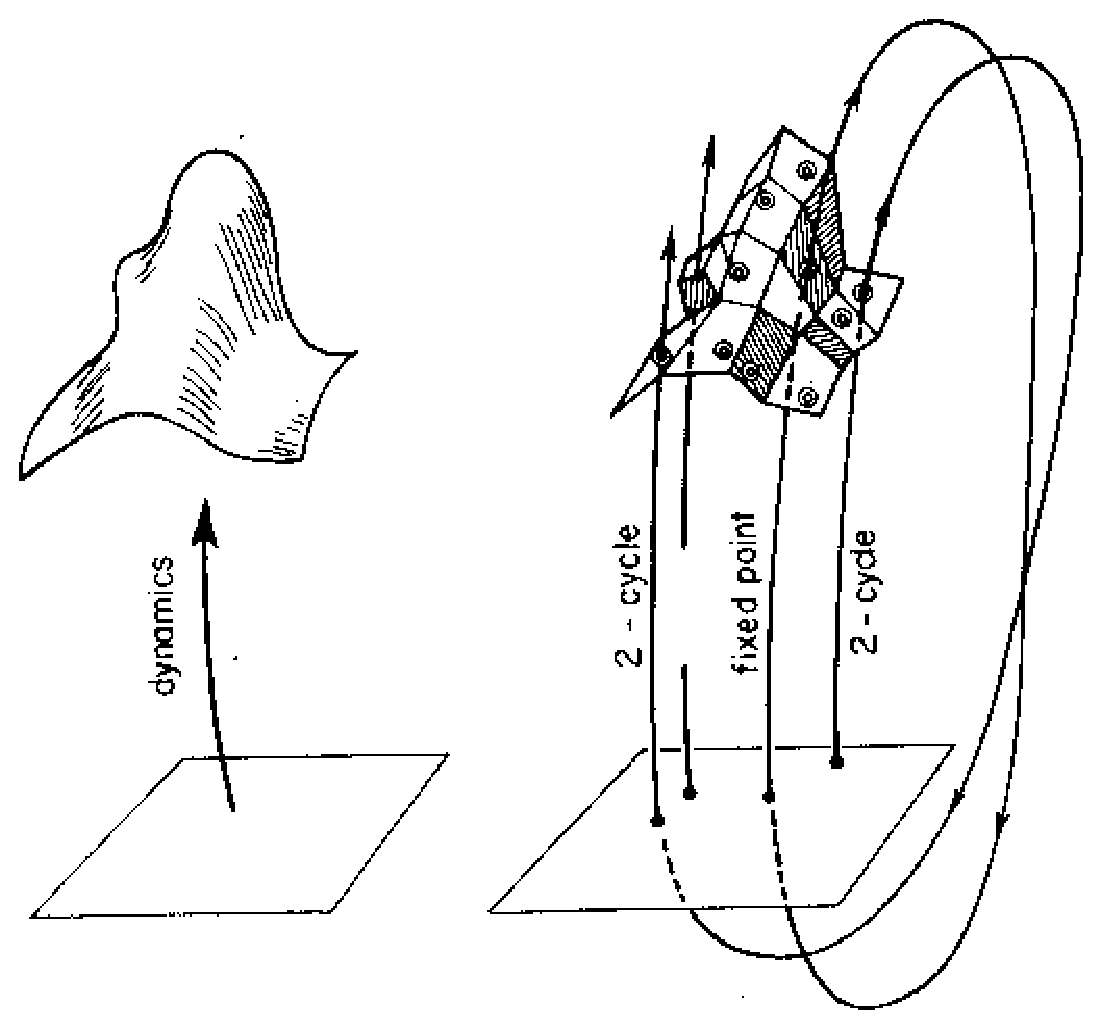
\includegraphics[width=0.60\textwidth]{f_1_08_1}
\end{center}
 tessellate the \statesp\ by {\Large recurrent flows}
\end{frame}

\begin{frame}{cartography for geometers}
\bigskip

\textcolor{blue}{cover the reduced manifold with a set of flat charts}

\hfill
\vfill
yes, we can do this with 8\dmn\ brick embedded in $10^6$ dimensions
\end{frame}

\begin{frame}{tiling the inertial manifold}
%%%%%%%%%% % \label{fig:CLf01group} %%%%%%%%%%%%%%
% 2011-09-09, 2012-03-30 Predrag: add BeThMovFr to
%            continuous.tex overheads, and ChaosBook
% replace A27movFrame*.* everywhere
  	\begin{center}
  	\setlength{\unitlength}{0.43\textwidth}
  \begin{picture}(1,0.94310243)%
    \put(0,0){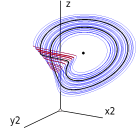
\includegraphics[width=\unitlength]{CLE1SliceSmall}}%
    \put(0.48564392,0.89244183){\color[rgb]{0,0,0}\makebox(0,0)[lb]{\smash{$z$}}}%
    \put(0.07181137,0.03185892){\color[rgb]{0,0,0}\makebox(0,0)[lb]{\smash{$y_2$}}}%
    \put(0.77031544,0.100183){\color[rgb]{0,0,0}\makebox(0,0)[lb]{\smash{$x_2$}}}%
  \end{picture}%
\quad
  	\setlength{\unitlength}{0.45\textwidth}
  \begin{picture}(1,1.05662086)%
    \put(0,0){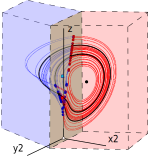
\includegraphics[width=\unitlength]{CLE2slicesmall}}%
    \put(0.47706962,0.83002768){\color[rgb]{0,0,0}\makebox(0,0)[lb]{\smash{$z$}}}%
    \put(0.08719004,0.02997825){\color[rgb]{0,0,0}\makebox(0,0)[lb]{\smash{$y_2$}}}%
    \put(0.73025395,0.09287946){\color[rgb]{0,0,0}\makebox(0,0)[lb]{\smash{$x_2$}}}%
  \end{picture}
    \end{center}

\bigskip
The N-chart atlas of the same
strange attractor stays in the physical manifold.

\end{frame}

\begin{frame}{linearized deterministic flow}

%%%%%%%%%%%%%%%%%%%%%%%%%%%%%%%%%%%%%%%%%%%%%%%%%
 \begin{center}
  \setlength{\unitlength}{0.65\textwidth}
  %% \unitlength = units used in the Picture Environment
  \begin{picture}(1,0.48527529)%
    \put(0,0){\includegraphics[width=\unitlength]{covariant1}}%
    \put(0.82300289,0.05462827){\color[rgb]{0,0,0}\rotatebox{0.03306771}{\makebox(0,0)[lb]{\smash{$\ssp_n$}}}}%
    \put(0.25001124,0.20377481){\color[rgb]{0,0,0}\rotatebox{0.03306771}{\makebox(0,0)[lb]{\smash{$\ssp_{n+1}$}}}}%
    \put(0.39195273,0.41066662){\color[rgb]{0,0,0}\rotatebox{0.03306771}{\makebox(0,0)[lb]{\smash{$\monodromy_n$}}}}%
    \put(0.89193475,0.41023002){\color[rgb]{0,0,0}\rotatebox{0.03306771}{\makebox(0,0)[lb]{\smash{$\vel_n$}}}}%
    \put(0.03306474,0.40112261){\color[rgb]{0,0,0}\rotatebox{0.03306771}{\makebox(0,0)[lb]{\smash{$\vel_{n+1}$}}}}%
  \end{picture}%
 \end{center}
%%%%%%%%%%%%%%%%%%%%%%%%%%%%%%%%%%%%%%%%%%%%%%%%%
\[
\ssp_{n+1} + \orbitDist_{n+1}= f(\ssp_n) + \monodromy_n \, \orbitDist_n
      \,, \quad
\monodromy_{ij} = \partial f_i / \partial \ssp_j
\]

\medskip

in one time step a linearized neighborhood of $\ssp_n$ is
\begin{enumerate}
	\item[(1)] advected by the flow
	\item[(2)]
transported by the \jacobianM\ $\monodromy_n$ into a
neighborhood given by the $\monodromy$
eigenvalues and eigenvectors
\end{enumerate}
\end{frame}

\begin{frame}{\rpo\ with a pair of Floquet vectors}
\begin{center}
\includegraphics[width=0.9\textwidth]{../../xiong/figures/rpo1_marginal}
\end{center}
\end{frame}

\begin{frame}{Floquet and Lyapunov exponents}
\begin{center}
\includegraphics[width=0.95\textwidth]{../../dimension/ks22FloqExp}
\end{center}
\end{frame}

\begin{frame}{entangled Floquet modes}
\begin{center}
\includegraphics[width=0.4\textwidth]{../../xiong/figures/localFEppo1}
\end{center}
\end{frame}

\begin{frame}{distribution of principal angles between Floquet subspaces}
\begin{center}
\includegraphics[width=0.7\textwidth]{../../dimension/ks22vecAngles}
\end{center}
\end{frame}

\begin{frame}{ergodic trajectory shadows \po s within the entangled subspace}
\begin{center}
\includegraphics[width=0.5\textwidth]{../../dimension/ks22vecShadow}
\end{center}
\end{frame}



\begin{frame}{what next? take the course!}
\begin{center}
\includegraphics[width=0.65\textwidth]{posterCB2cover}
\end{center}
\vfill
student raves : \\
...$10^6$ times harder than any other online course...
\end{frame}








% leftovers:


\end{document}
